% --- BẮT ĐẦU NỘI DUNG part3_paper1.tex ---

\subsection{Phân tích bài báo: Bipartite Ranking through Minimization of Univariate Loss}

\textbf{Thông tin nghiên cứu:} Bài báo của Kotłowski, Dembczyński, và Hüllermeier công bố tại hội nghị ICML (2011).

\subsubsection{Giới thiệu và bối cảnh bài báo}

Bài báo đặt ra và giải quyết một câu hỏi cốt lõi có ý nghĩa thực tiễn lớn trong bài toán phân hạng:

\begin{quote}
\textbf{Câu hỏi nghiên cứu trung tâm:} \textit{Chúng ta mất bao nhiêu hiệu suất xếp hạng (ranking performance) khi huấn luyện một bộ phân loại đơn giản -- tối thiểu hóa hàm mất mát đơn biến (univariate loss) trên dữ liệu gốc -- thay vì huấn luyện trực tiếp một bộ xếp hạng trên các cặp điểm?}
\end{quote}

Đây là câu hỏi có tầm quan trọng vì:
\begin{enumerate}
  \item Bài toán \textbf{xếp hạng bipartite} (bipartite ranking) -- xếp hạng các điểm dương cao hơn các điểm âm -- có hàm mục tiêu được định nghĩa trên \emph{tất cả các cặp} (dương, âm). Số cặp này là $O(mn)$, dẫn đến độ phức tạp tính toán bậc hai theo cỡ mẫu.
  \item Ngược lại, các thuật toán phân loại tiêu chuẩn tối thiểu hóa hàm mất mát \emph{đơn biến} (univariate), tức là tính trên từng điểm riêng lẻ, có độ phức tạp chỉ $O(n)$ hoặc $O(n \log n)$.
  \item Thực nghiệm trước đó cho thấy các bộ phân loại đơn giản -- nhất là những bộ tối thiểu hóa hàm mất mát margin -- thực hiện khá tốt về AUC. Bài báo này cung cấp nền tảng lý thuyết giải thích hiện tượng đó.
\end{enumerate}

\subsubsection{Thiết lập và ký hiệu}

\textbf{Bài toán phân loại nhị phân:} Cho cặp ngẫu nhiên $(x, y) \in \mathcal{X} \times \{-1, +1\}$ được sinh theo phân phối $P(x, y)$. Một bộ phân loại $c: \mathcal{X} \to \mathbb{R}$ có rủi ro phân loại (classification risk):
\begin{equation}
  L_\ell(c) := \mathbb{E}\bigl[\ell(y,\, c(x))\bigr]
\end{equation}
với $\ell: \{-1,+1\} \times \mathbb{R} \to \mathbb{R}_{\geq 0}$ là hàm mất mát. Hối tiếc (regret) của $c$ được định nghĩa là khoảng cách từ rủi ro của $c$ đến rủi ro của bộ phân loại Bayes tối ưu.

\textbf{Định nghĩa (Xếp hạng bipartite):} Mục tiêu là học một hàm $c: \mathcal{X} \to \mathbb{R}$ sao cho $c(x') > c(x)$ với mọi $x'$ dương và $x$ âm với xác suất cao nhất. 

Rủi ro xếp hạng (rank risk) đo lường xác suất xếp sai thứ tự một cặp:
\begin{equation}
  L_{\text{rank}}(r) := \mathbb{P}\bigl(r(x, x') = -1 \mid y > y'\bigr) + \frac{1}{2}\mathbb{P}\bigl(r(x, x') = 0 \mid y > y'\bigr)
\end{equation}
với $x$ và $x'$ là các mẫu độc lập. Bộ xếp hạng Bayes có dạng $r^*(x, x') = \text{sgn}\bigl(\eta(x) - \eta(x')\bigr)$, trong đó $\eta(x) = \mathbb{P}(y=1 \mid x)$.

\begin{quote}
\textbf{Liên hệ với lý thuyết (Chương 9):}
Định nghĩa về rủi ro xếp hạng và bộ xếp hạng Bayes hoàn toàn nhất quán với định nghĩa trong Mục 9.5, Chương 9. Tuy nhiên, bài báo bổ sung thêm khái niệm \emph{hối tiếc xếp hạng} (rank regret) -- một chỉ số mạnh hơn đo lường khoảng cách đến hiệu suất tối ưu mà giáo trình chưa xoáy sâu.
\end{quote}

\subsubsection{Trường hợp Hàm mất mát 0/1}

\textbf{Bổ đề:} Cho bộ phân loại $c$. Đặt $\alpha$ là xác suất âm giả, $\beta$ là xác suất dương giả và $p = \mathbb{P}(y=+1)$. Khi đó rủi ro phân hạng bị chặn bởi:
\begin{equation}
  L_{\text{rank}}(c) \leq \frac{\alpha}{p} + \frac{\beta}{1-p} - \alpha\beta\, p(1-p)
\end{equation}

Từ bổ đề trên, bài báo rút ra định lý giới hạn rủi ro cho hàm mất mát 0/1.

\textbf{Định lý 1 (Chặn rủi ro 0/1 loss):} Với phân phối có xác suất lớp dương $p$, mọi bộ phân loại $c$ đều thỏa mãn:
\begin{equation}
  L_{\text{rank}}(c) \leq \frac{L_{0/1}(c)}{\min\{p,\, 1-p\}}
\end{equation}

\begin{quote}
\textbf{Nhận xét:} Chặn này cho thấy tối ưu rủi ro phân loại sẽ giúp tối ưu rủi ro phân hạng. Tuy nhiên, nếu lớp dữ liệu mất cân bằng nặng (ví dụ $p \to 0$), hằng số $1/\min\{p, 1-p\}$ sẽ rất lớn, khiến chặn này trở nên lỏng lẻo. Để khắc phục, tác giả đề xuất sử dụng hàm mất mát 0/1 được cân bằng trọng số.
\end{quote}

\subsubsection{Trường hợp Hàm mất mát Margin}

Đây là kết quả cốt lõi của bài báo, chứng minh rằng các hàm mất mát margin (như exponential trong AdaBoost hay logistic trong Logistic Regression) có những tính chất vượt trội cho bài toán phân hạng.

\textbf{Định lý 2 (Chặn hối tiếc - Exponential và Logistic Loss):} 
Cho $\ell$ là hàm mất mát margin cân bằng trọng số. Hối tiếc xếp hạng $\text{Reg}_{\text{rank}}(c)$ bị chặn bởi:
\begin{align}
  \text{Reg}_{\text{rank}}(c) &\leq \frac{3\sqrt{2}}{2}\sqrt{\text{Reg}_{\exp}(c)} \quad \text{(với hàm exponential)} \\
  \text{Reg}_{\text{rank}}(c) &\leq 2\sqrt{\text{Reg}_{\log}(c)} \quad \text{(với hàm logistic)}
\end{align}

\begin{quote}
\textbf{Liên hệ với lý thuyết (Chương 9):}
Chứng minh của bài báo sử dụng \textbf{kỹ thuật rút gọn} xếp hạng về phân loại bằng cách tạo không gian mới gồm các cặp mẫu $\tilde{x} = (x, x')$. Đây chính là kỹ thuật nền tảng được dùng trong Chương 9 để xây dựng thuật toán RankSVM (Mục 9.3) và RankBoost (Mục 9.4). Đặc biệt, bài báo đã chứng minh được tính \emph{nhất quán} -- tức là hối tiếc của các hàm mục tiêu này tiến về 0 sẽ kéo theo hối tiếc phân hạng tiến về 0.
\end{quote}

\subsubsection{Thực nghiệm kiểm chứng}

Bài báo so sánh ba thuật toán trên các tập dữ liệu thực (tất cả đều dùng mô hình tuyến tính với L2 regularization):
\begin{enumerate}
  \item \textbf{Exponential loss} (tương tự thuật toán boosting).
  \item \textbf{Logistic loss} (hồi quy logistic).
  \item \textbf{Pairwise hinge loss} (thuật toán SVM-OR tối ưu hóa trực tiếp trên $O(mn)$ cặp mẫu).
\end{enumerate}

\begin{table}[H]
  \centering
  \caption{Rủi ro phân hạng trên một số bộ dữ liệu thực. Giá trị nhỏ hơn là tốt hơn.}
  \vspace{0.2cm}
  \begin{tabular}{lccc}
    \toprule
    \textbf{Bộ dữ liệu} & \textbf{Exponential} & \textbf{SVM-OR} & \textbf{Logistic} \\
    \midrule
    Breast-w  & 0.0051 & \textbf{0.0049} & 0.0054 \\
    Colic     & 0.1251 & 0.1352 & \textbf{0.1179} \\
    Diabetes  & 0.1724 & \textbf{0.1702} & 0.1804 \\
    Ionosphere& 0.0811 & \textbf{0.0773} & 0.0884 \\
    Covtype   & 0.1635 & \textbf{0.1604} & 0.1623 \\
    \bottomrule
  \end{tabular}
\end{table}

\textbf{Nhận xét kết quả:}
Thuật toán SVM-OR (tương đương RankSVM trong Mục 9.3) đôi khi cho kết quả tốt hơn nhưng độ chênh lệch vô cùng nhỏ. Đặc biệt, \textbf{Logistic loss cạnh tranh ngang ngửa} với SVM-OR dù chỉ cần độ phức tạp tính toán $O(n)$ thay vì $O(mn)$. Điều này xác nhận về mặt thực nghiệm các luận điểm lý thuyết: tối thiểu hóa hàm mất mát đơn biến phù hợp hoàn toàn có khả năng phân hạng xuất sắc.

\subsubsection{Đánh giá phê bình và hướng mở rộng}

\textbf{Điểm mạnh:}
\begin{itemize}
    \item Cung cấp nền tảng lý thuyết vững chắc (chứng minh chặt chẽ cả chặn rủi ro và chặn hối tiếc) giải thích tại sao các thuật toán như hồi quy logistic lại tối ưu AUC rất tốt trong thực tế.
    \item Gợi ý một giải pháp thực tiễn có khả năng thay thế các phương pháp tiếp cận pairwise phức tạp, giúp giảm chi phí tính toán rõ rệt.
\end{itemize}

\textbf{Hạn chế \& Câu hỏi mở:}
\begin{itemize}
    \item Các hằng số trong chặn hối tiếc có thể vẫn chưa phải là tối ưu nhất.
    \item Các phân tích tập trung chủ yếu ở cấp độ phân phối xác suất (population level), chưa đi sâu vào tốc độ hội tụ hữu hạn mẫu (finite-sample) như một số định lý trong Chương 9.
    \item Cần thêm nghiên cứu để mở rộng bài toán sang các bối cảnh phức tạp hơn như k-partite ranking hoặc áp dụng trên các tiêu chuẩn đo lường tối ưu công cụ tìm kiếm như NDCG.
\end{itemize}

\subsubsection{Demo thử nghiệm}

Để làm rõ hơn luận điểm của bài báo, nhóm đã tiến hành xây dựng một thực nghiệm mô phỏng bằng Python. Mục tiêu là so sánh trực tiếp hai hướng tiếp cận trên một tập dữ liệu mất cân bằng nghiêm trọng (100 mẫu dương tính và 1000 mẫu âm tính):

\begin{enumerate}
    \item \textbf{Mô hình Univariate (Logistic Regression):} Tối ưu hóa hàm Logistic Loss trên 1100 điểm dữ liệu độc lập, độ phức tạp $O(m+n)$.
    \item \textbf{Mô hình Pairwise (Hinge Loss qua PyTorch):} Tối ưu hóa Margin Ranking Loss bằng cách xét duyệt toàn bộ không gian 100,000 cặp dữ liệu, độ phức tạp $O(mn)$.
\end{enumerate}

\begin{figure}[H]
    \centering
    % Đảm bảo ảnh roc_curve_comparison.png nằm trong thư mục figures cùng cấp với file main.tex
    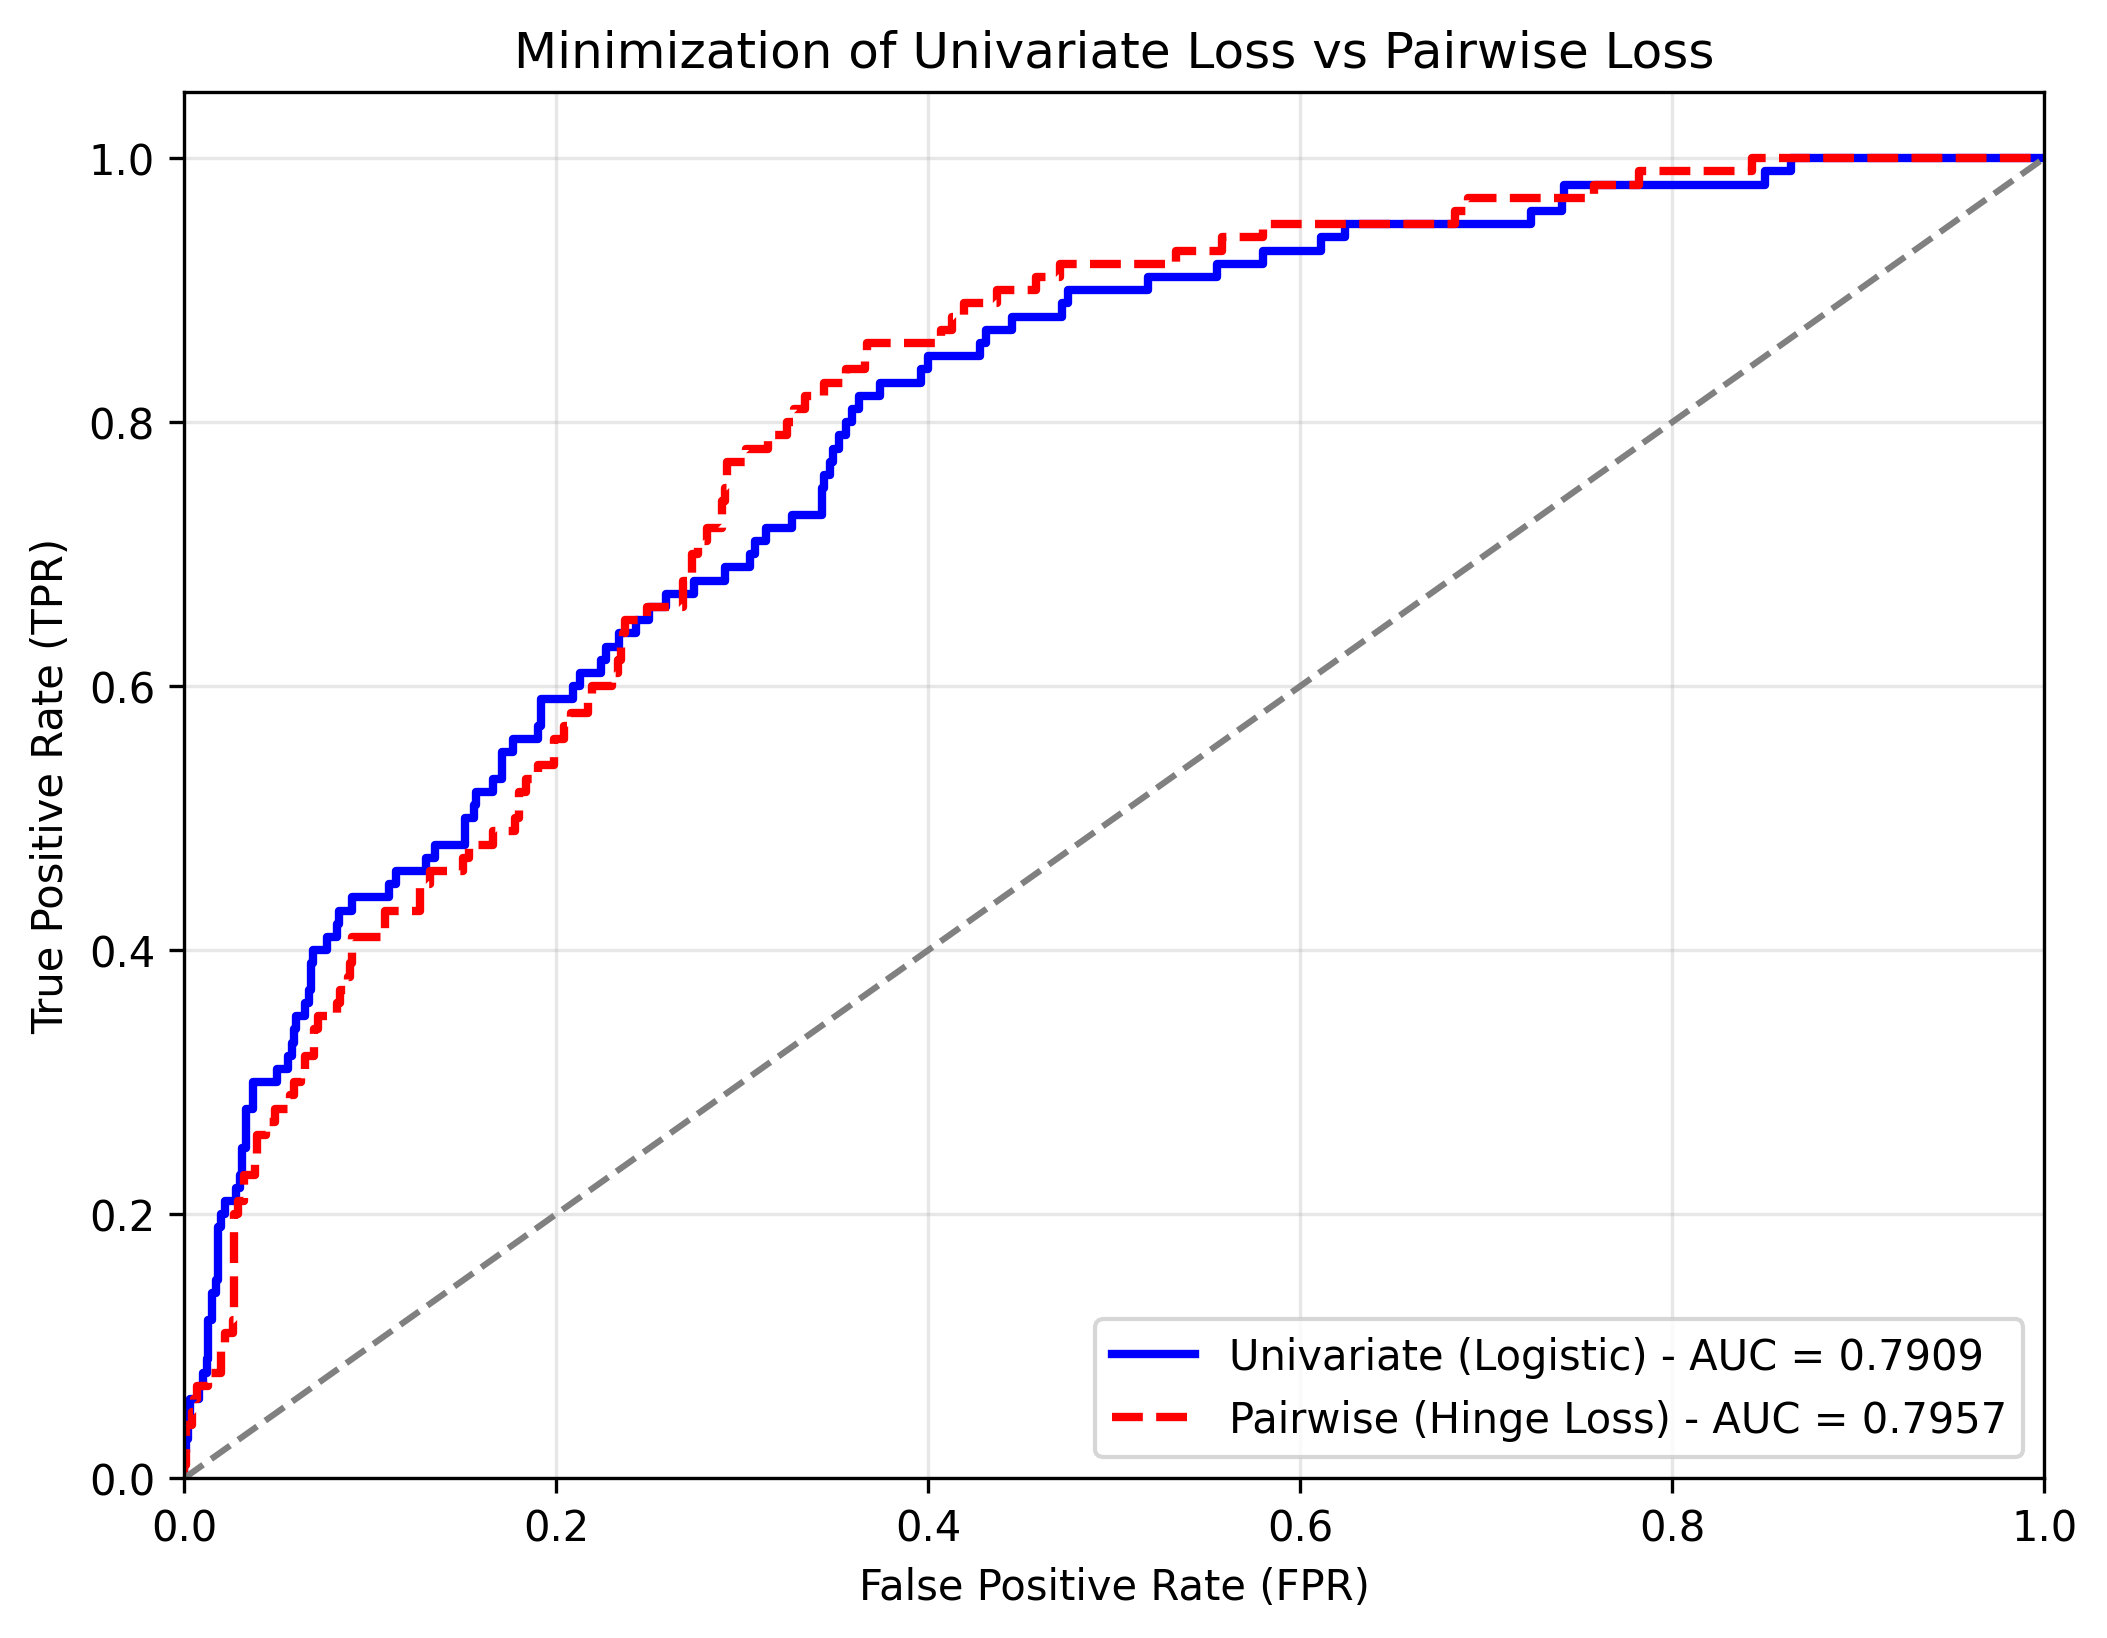
\includegraphics[width=0.8\textwidth]{figures/roc_curve_comparison.png}
    \caption{Đường cong ROC so sánh hiệu suất giữa mô hình Univariate và Pairwise trên tập dữ liệu mô phỏng mất cân bằng.}
    \label{fig:roc_comparison}
\end{figure}

\textbf{Kết luận từ thực nghiệm:} 
Như quan sát trên Hình \ref{fig:roc_comparison}, mặc dù mô hình Univariate hoàn toàn không sử dụng thông tin bắt cặp và được huấn luyện trên dữ liệu mất cân bằng nặng (tỷ lệ 10:1), nó vẫn đạt được chỉ số xếp hạng $\text{AUC} \approx 0.7909$, gần như bám sát và cạnh tranh sòng phẳng với mức $\text{AUC} \approx 0.7957$ của phương pháp Pairwise truyền thống. Kết quả này phản ánh chính xác Định lý của bài báo: tối thiểu hóa hàm mất mát margin đơn biến là một công cụ mạnh mẽ, ổn định và tiết kiệm tài nguyên tính toán cho bài toán phân hạng Bipartite.

% --- KẾT THÚC NỘI DUNG part3_paper1.tex ---